\documentclass{article}
\usepackage[utf8]{inputenc}
\usepackage[T1]{fontenc}
\usepackage[english, polish]{babel}
\usepackage{geometry}
\usepackage{graphicx}
\usepackage{float}
\usepackage{hyperref}
\usepackage{listings}
\usepackage{appendix}
\usepackage{titlesec}
\usepackage{biblatex}
\usepackage{xcolor}

\addbibresource{bibliografia.bib}



\title{Zgadywanka - Gra z Obrazkami \\ \Large{Sprawozdanie Projektowe}}
\author{Julia Hryciuk, Mateusz Drozd, Jakub Kalita}

\begin{document}

	\maketitle
	\begin{figure}[H]
		\centering
		
\includegraphics[width=0.8\linewidth]{Ikona.jpg}
	\end{figure}

\tableofcontents
\newpage
	\section{Wstęp}
	W dzisiejszych czasach tworzenie gier komputerowych staje się coraz bardziej popularne i dostępne. Celem tego projektu było stworzenie prostej, interaktywnej gry w języku C++, żeby rozwijać umiejętności praktyczne w zakresie programowania.
	
	\section{Streszczenie}
	% Krótkie streszczenie projektu.
	
	Projekt "Zgadywanka" to gra polegająca na odgadywaniu obrazków. Na planszy ukazane jest 12 elementów, z których co pewien czas odsłania się jeden. Gracz musi zgadnąć, co przedstawia obrazek, korzystając z okna odpowiedzi. Po udanej odpowiedzi wyświetla się komunikat o poprawnej odpowiedzi, a gracz może rozpocząć nową grę z losowym obrazkiem. Po niepoprawnej  odowiedzi wyswietla sie komunikat o błędzie, a gracz musi zgadywać dalej. Gra została zaimplementowana w środowisku Code::Blocks, wykorzystując podstawy programowania obiektowego.
	
	
	\section{Cel Projektu}
	% Szczegółowy opis celów projektu.
	
	Główne cele projektu obejmowały:
	\begin{itemize}
		\item Implementację interaktywnej planszy z elementami.
		\item Losowe odsłanianie obrazków co kilka sekund.
		\item Możliwość udzielenia odpowiedzi przez gracza.
		\item Obsługę poprawnych i błędnych odpowiedzi.
		\item Losowanie nowych obrazków po poprawnej odpowiedzi.
		\item Ustawienie czasu, aby gracz wiedział jak szybko udaje mu sie podac prawidłową odpowiedź.
	\end{itemize}
	\section{Struktura Katalogów: Zgadywanka}
	% Opis struktury katalogów w projekcie.
	
	Struktura katalogów projektu Zgadywanka jest zorganizowana w następujący sposób:
	\begin{itemize}
		\item \texttt{Zgadywanka/}
		\begin{itemize}
			\item \texttt{src/} - Kod źródłowy aplikacji.
			\item \texttt{images/} - Zasoby graficzne (obrazki).
			\item \texttt{docs/} - Dokumentacja projektu.
			\item \texttt{install/} - Pliki instalacyjne.
		\end{itemize}
	\end{itemize}
	
		\section{Opis Aplikacji}
	% Szczegółowy opis funkcji aplikacji.
	
	Aplikacja prezentuje interaktywną planszę z elementami, z których jeden co jakiś czas odsłania się na krótko. Gracz musi odgadnąć, co przedstawia obrazek, wpisując odpowiedź w oknie przewidzianym do tego celu. Po poprawnej odpowiedzi wyświetla się komunikat, a gracz ma możliwość rozpoczęcia nowej gry z losowym obrazkiem. W przypadku błędnej odpowiedzi czas się nie zatrzymuje, a gracz może próbować ponownie.
	
	\section{Jak wygląda gra}
	
	\subsection{Podczas Gry}
	\begin{figure}[H]
		\centering
		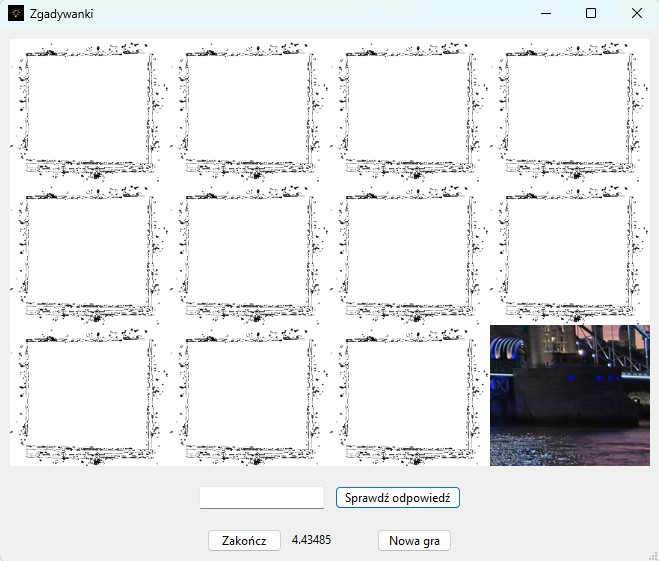
\includegraphics[width=0.8\linewidth]{zrzut_gry.jpg}
		\caption{Zrzut ekranu podczas trwania gry.}
		\label{fig:gry}
	\end{figure}
	
	\subsection{Po Poprawnej Odpowiedzi}
	\begin{figure}[H]
		\centering
		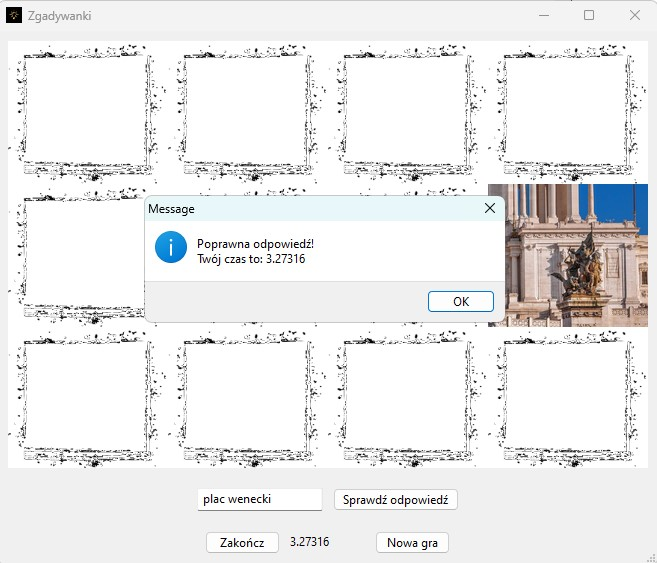
\includegraphics[width=0.8\linewidth]{poprawna_odp.jpg}
		\caption{Zrzut ekranu po udzieleniu poprawnej odpowiedzi.}
		\label{fig:poprawna_odp}
	\end{figure}
	
	\subsection{Po Błędnej Odpowiedzi}
	\begin{figure}[H]
		\centering
		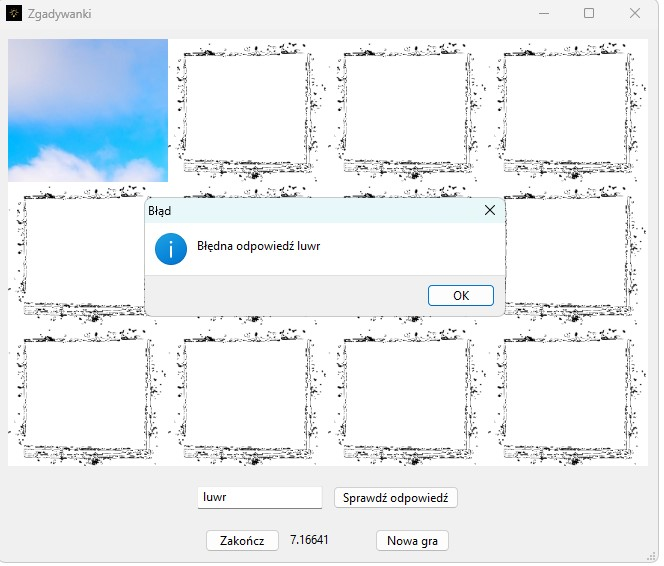
\includegraphics[width=0.8\linewidth]{bledna_odp.jpg}
		\caption{Zrzut ekranu po udzieleniu błędnej odpowiedzi.}
		\label{fig:bledna_odp}
	\end{figure}
	
	
	\section{Implementacja}
	% Opis implementacji kluczowych funkcji.
	
	\subsection{Implementację interaktywnej planszy z elementami}
	% Fragmenty kodu związane z odsłanianiem elementów.

\lstset{
	language=C++,
	basicstyle=\ttfamily, 
	numbers=left, 
	numberstyle=\tiny, 
	stepnumber=1, 
	keywordstyle=\color{blue}\bfseries,
	commentstyle=\color{green!60!black},
	identifierstyle=\color{black},
	stringstyle=\color{orange},
	numbersep=5pt, 
	showspaces=false, 
	showstringspaces=false, 
	showtabs=false, 
	frame=single,
	tabsize=2,
	captionpos=b, 
	breaklines=true, 
	breakatwhitespace=true, 
	escapeinside={\%*}{*)},
	literate=%
	{ą}{{\k{a}}}1
	{ć}{{'c}}1
	{ę}{{\k{e}}}1
	{ł}{{\l{}}}1
	{ń}{{'n}}1
	{ó}{{'o}}1
	{ś}{{'s}}1
	{ż}{{.z}}1
	{ź}{{'z}}1
	{Ą}{{\k{A}}}1
	{Ć}{{'C}}1
	{Ę}{{\k{E}}}1
	{Ł}{{\L{}}}1
	{Ń}{{'N}}1
	{Ó}{{'O}}1
	{Ś}{{'S}}1
	{Ż}{{.Z}}1
	{Ź}{{'Z}}1
}

	
	
	Poniżej przedstawiono fragment kodu odpowiedzialnego za odsłanianie elementów na planszy:
	\begin{lstlisting}
		wxStaticBitmap* pola[16];
		wxBitmap rysunki[4];
		std::map <int,int> id2nr;
		zgadywanka gra;
		int licznik=0;
		int numer_obrazka = (rand() % 17);
		int b=numer_obrazka;
		
		std::string nazwa_obrazka = "zdjecia/"+std::to_string(numer_obrazka+1)+".png";
		
		wxBitmap zakryj(int k = -1);
		
		
		wxBitmap obrazek, obrazek_zakryty;
	\end{lstlisting}

	\begin{lstlisting}
		wxBitmap ProjectDialog::zakryj(int k) {
			wxBitmap tmp = obrazek;
			wxMemoryDC dc;
			dc.SelectObject(tmp);
			for (int i = 0; i < 16; ++i) {
				if (k==i)
				continue;
				int x = (i % 4) * 160;
				int y = (i / 4) * 143;
				dc.DrawBitmap(wxImage("kwadracik.png"), wxPoint(x, y));
			}
			dc.SelectObject(wxNullBitmap);
			return tmp;
		}
	\end{lstlisting}
	
	\subsection{Losowe odsłninie obrazów co 50 sekund}
	% Fragmenty kodu związane z obsługą odpowiedzi gracza.
	
	Poniżej przedstawiono fragment kodu odpowiedzialnego za losowe odsłninie obrazów co kilka sekund :
	
	\begin{lstlisting}
		void ProjectDialog::OnTimer1Trigger(wxTimerEvent& event)
		{
			licznik++;
			double c = licznik * Timer1.GetInterval() / 1274.0;
			wxString czas;
			czas << c;
			StaticText1->SetLabel(czas);
			if(licznik ==6368){
				Timer1.Stop();
				Timer2.Stop();
				wxString answersFilePath = wxT("Rozwiazania.txt"); // Zmień na właściwą ścieżkę do pliku
				wxTextFile file;
				if (file.Open(answersFilePath)) {
					
					// Sprawdź, czy numer linii odpowiada numerowi obrazka
					
					
					wxString correctAnswer = file.GetLine(numer_obrazka);
					correctAnswer = correctAnswer.Lower();
					
					// Pobierz wpisaną przez użytkownika odpowiedź
					wxString enteredText = TextCtrl1->GetValue();
					enteredText = _(enteredText.Lower());
					// Porównaj odpowiedź z poprawną odpowiedzią z pliku
					wxMessageBox(_("Nowy obrazek zostanie wczytany \nTwój czas to "+ czas));
					numer_obrazka = (rand() % 17);
					while(b==numer_obrazka){
						
						numer_obrazka = (rand() % 17);
					}
					std::string nazwa_obrazka = "zdjecia/"+std::to_string(numer_obrazka+1)+".png";
					StaticBitmap2->SetBitmap(wxImage(nazwa_obrazka));
					obrazek = StaticBitmap2->GetBitmap();
					obrazek_zakryty = zakryj();
					StaticBitmap2->SetBitmap(obrazek_zakryty);
					TextCtrl1->Clear();
					licznik=0;
					Timer2.Start();
					Timer1.Start();
					
				}
			}
		}
	\end{lstlisting}
	
	\subsection{Możliwość udzielenia odpowiedzi przez grcza}
	Poniżej przedstawiono fragment kodu odpowiedzialnego za możliwość udzielenia odpowiedzi przez grcza:
	\begin{lstlisting}
	void ProjectDialog::OnTimer2Trigger(wxTimerEvent& event)
	{
		int k = rand() % 12;
		auto obrazek = zakryj(k);
		StaticBitmap2->SetBitmap(obrazek);
	}
	\end{lstlisting}
	
	\subsection{Obsługa poprawnyh i błędnych opowiedzi}
	Poniżej przedstawiono fragment kodu odpowiedzialnego za obsługa poprawnyh i błędnych opowiedzi:
	\begin{lstlisting}
		void ProjectDialog::OnButton2Click(wxCommandEvent& event)
		
		{
			
			// Utwórz nazwę pliku tekstowego zawierającego odpowiedzi
			wxString answersFilePath = wxT("Rozwiazania.txt"); // Zmień na właściwą ścieżkę do pliku
			Timer1.Stop();
			Timer2.Stop();
			// Otwórz plik tekstowy
			double c = licznik * Timer1.GetInterval() / 1274.0;
			wxString czas;
			czas << c;
			wxTextFile file;
			
			if (file.Open(answersFilePath)) {
				
				// Sprawdź, czy numer linii odpowiada numerowi obrazka
				
				
				wxString correctAnswer = file.GetLine(numer_obrazka);
				correctAnswer = correctAnswer.Lower();
				
				// Pobierz wpisaną przez użytkownika odpowiedź
				
				wxString enteredText = TextCtrl1->GetValue();
				enteredText = enteredText.Lower();
				// Porównaj odpowiedź z poprawną odpowiedzią z pliku
				
				if (enteredText == correctAnswer) {
					wxMessageBox(_("Poprawna odpowiedź! \nTwój czas to: "+czas));
					
					wxMessageBox("Nowy obrazek zostanie wczytany");
					numer_obrazka = (rand() % 17);
					while(b==numer_obrazka){
						
						numer_obrazka = (rand() % 17);
					}
					std::string nazwa_obrazka = "zdjecia/"+std::to_string(numer_obrazka+1)+".png";
					
					wxString correctAnswer = file.GetLine(numer_obrazka);
					correctAnswer = correctAnswer.Lower();
					
					StaticBitmap2->SetBitmap(wxImage(nazwa_obrazka));
					obrazek = StaticBitmap2->GetBitmap();
					obrazek_zakryty = zakryj();
					StaticBitmap2->SetBitmap(obrazek_zakryty);
					licznik=0;
					Timer1.Start();
					Timer2.Start();
				}
				
				else {
					
					wxMessageBox(_("Błędna odpowiedź: "+ enteredText), _("Błąd"));
					Timer1.Start();
					Timer2.Start();
				}
				
				
				
				TextCtrl1->Clear();
					}
				}
		
	\end{lstlisting}
	
	\subsection{Losowanie nowyh obrazków po udzieleniu poprawnej odpowiedzi}
	Poniżej przedstawiono fragment kodu odpowiedzialnego za losowanie nowyh obrazków po udzieleniu poprawnej odpowiedzi:
	\begin{lstlisting}
		if (enteredText == correctAnswer) {
			wxMessageBox(_("Poprawna odpowiedź! \nTwój czas to: "+czas));
			
			wxMessageBox("Nowy obrazek zostanie wczytany");
			numer_obrazka = (rand() % 17);
			while(b==numer_obrazka){
				
				numer_obrazka = (rand() % 17);
			}
			std::string nazwa_obrazka = "zdjecia/"+std::to_string(numer_obrazka+1)+".png";
			
			wxString correctAnswer = file.GetLine(numer_obrazka);
			correctAnswer = correctAnswer.Lower();
			
			StaticBitmap2->SetBitmap(wxImage(nazwa_obrazka));
			obrazek = StaticBitmap2->GetBitmap();
			obrazek_zakryty = zakryj();
			StaticBitmap2->SetBitmap(obrazek_zakryty);
			licznik=0;
			Timer1.Start();
			Timer2.Start();
		}
	\end{lstlisting}
	
	\subsection{Ustawienie czasu, aby gracz wiedział jak szybko udaje mu sie podać poprawn odpowiedź oraz losowanie nowego obrazka po 50 sekundach gry}
	Poniżej przedstawiono fragment kodu odpowiedzialnego za ustawienie czasu, aby gracz wiedział jak szybko udaje mu sie podać poprawną odpowiedź:
	\begin{lstlisting}
		void ProjectDialog::OnButton3Click(wxCommandEvent& event)
		{
			Timer1.Stop();
			Timer2.Stop();
			wxString answersFilePath = wxT("Rozwiazania.txt");
			wxTextFile file;
			wxMessageBox("Nowy obrazek zostanie wczytany");
			numer_obrazka = (rand() % 17);
			while(b==numer_obrazka){
				
				numer_obrazka = (rand() % 17);
			}
			b=numer_obrazka;
			std::string nazwa_obrazka = "zdjecia/"+std::to_string(numer_obrazka+1)+".png";
			StaticBitmap2->SetBitmap(wxImage(nazwa_obrazka));
			obrazek = StaticBitmap2->GetBitmap();
			obrazek_zakryty = zakryj();
			StaticBitmap2->SetBitmap(obrazek_zakryty);
			TextCtrl1->Clear();
			licznik = 0;
			Timer1.Start();
			Timer2.Start();
			
			
			
		}
	\end{lstlisting}
	

	
	\section{Program Instalacyjny}
	% Opis procesu instalacji aplikacji.
	
	Aby zainstalować aplikację Zgadywanka, wykonaj następujące kroki:
	\begin{enumerate}
		\item Przejdź do katalogu \texttt{install/}.
		\item Uruchom plik instalacyjny \texttt{install.sh}.
		\item Postępuj zgodnie z instrukcjami na ekranie.
	\end{enumerate}
	\section{Problemy napotkane podczas tworzenia aplikacji}


Podczas procesu tworzenia aplikacji "Zgadywanka" napotkaliśmy pewne wyzwania, które wymagały dodatkowej uwagi i rozważań. Poniżej przedstawiamy szczegółowy opis tych problemów.

\subsection{Problemy z Kwadratami}

\begin{enumerate}
	\item \textbf{Przesłanianie Kwadratów:} W trakcie implementacji zauważyliśmy, że kwadraty, reprezentujące elementy gry, czasami nakładają się na siebie w sposób, który nie spełnia naszych oczekiwań estetycznych. To zjawisko wymagało dodatkowej uwagi w zakresie warstw i pozycjonowania kwadratów, aby osiągnąć pożądany efekt wizualny.
	
	\item \textbf{Animacja Odsłaniania:} Kolejnym problemem było zapewnienie płynnej animacji odsłaniania kwadratów. Choć podstawowa logika animacji została zaimplementowana, pojawiły się wyzwania związane z optymalizacją tego procesu, aby uzyskać satysfakcjonujący efekt wizualny.
\end{enumerate}

\subsection{Problemy z Czytaniem Małych i Dużych Liter}

\begin{enumerate}
	\item \textbf{Weryfikacja Wielkości Liter:} W funkcji odpowiedzialnej za odczyt liter, napotkaliśmy trudności z prawidłowym rozróżnieniem między małymi a dużymi literami. Było istotne stworzenie mechanizmu weryfikującego wielkość liter, aby poprawnie interpretować odpowiedzi użytkownika.
	
	\item \textbf{Normalizacja Wielkości Liter:} Dodatkowym wyzwaniem było zagwarantowanie spójności w interpretacji liter bez względu na ich wielkość. Zastosowaliśmy funkcje dostępne w języku C++.
\end{enumerate}

	\section{Podział pracy}
\begin{itemize}
	\item \textbf {Julia Hryciuk} .
	\item \textbf {Mateusz Drozd} .
	\item \textbf {Jakub Kalita} .
\end{itemize}
	\section{Podziękowania}
	Chcielibyśmy podziękować naszemu opiekunowi projektu za cenne wskazówki i wsparcie w trakcie realizacji zadania.
	
	\section{Bibliografia}
\begin{itemize}
	\item https://wiki.codeblocks.org/index.php/WxSmithtutorial:Helloworld
	
	\item https://fly.pl/aktualnosci/grecja-po-pozarach-bezpieczne-wakacje-w-grecji/

	\item https://pl.wikipedia.org/wiki/D%C5%BCenne
	
	\item https://motozwiedzanie.pl/palac-wenecki-klejnot-wiecznego-miasta/

	\item https://www.national-geographic.pl/traveler/artykul/luwr-ma-juz-230-lat-to-najchetniej-odwiedzane-muzeum-swiata

	\item https://www.unesco.pl/kultura/dziedzictwo-kulturowe/swiatowe-dziedzictwo/lista-swiatowego-dziedzictwa/
	

\end{itemize}
\end{document}
